\documentclass[conference]{IEEEtran}
\IEEEoverridecommandlockouts
% The preceding line is only needed to identify funding in the first footnote. If that is unneeded, please comment it out.
\usepackage{amsmath,amssymb,amsfonts}
\usepackage{algorithmic}
\usepackage{graphicx}
\usepackage[inline, shortlabels]{enumitem}
\usepackage{tabularx}
\usepackage{caption}
\usepackage{titlesec}
\usepackage[T2A,T1]{fontenc}
\usepackage[english]{babel}
\captionsetup{font=it}
\usepackage{ragged2e}
\usepackage{hyperref}
\addto\extrasenglish{%
  \renewcommand{\sectionautorefname}{Section}%
  \renewcommand{\subsectionautorefname}{Subsection}%
  \renewcommand{\subsubsectionautorefname}{Subsubsection}%
  \renewcommand{\tableautorefname}{Table}%
  \renewcommand{\figureautorefname}{Figure}%
}
\usepackage{pifont}
\newcommand{\cmark}{\ding{51}}%
\newcommand{\xmark}{\ding{55}}%
\usepackage{footmisc}
\usepackage{multirow}

% --- Tickz
\usepackage{physics}
\usepackage{amsmath}
\usepackage{tikz}
\usepackage{mathdots}
\usepackage{yhmath}
\usepackage{cancel}
\usepackage{color}
\usepackage{siunitx}
\usepackage{array}
\usepackage{multirow}
\usepackage{amssymb}
\usepackage{gensymb}
\usepackage{tabularx}
\usepackage{extarrows}
\usepackage{booktabs}
\usetikzlibrary{fadings}
\usetikzlibrary{patterns}
\usetikzlibrary{shadows.blur}
\usetikzlibrary{shapes}

% ---------

\usepackage{pdfpages}
\usepackage{booktabs}
\usepackage{csquotes}
\usepackage{lipsum}  
\usepackage{arydshln}
\usepackage{smartdiagram}
\usepackage[inkscapeformat=png]{svg}
\usepackage{textcomp}
\usepackage{tabularray}\UseTblrLibrary{varwidth}
\usepackage{xcolor}
\def\BibTeX{{\rm B\kern-.05em{\sc i\kern-.025em b}\kern-.08em
    T\kern-.1667em\lower.7ex\hbox{E}\kern-.125emX}}
\usepackage{cite}
\usepackage{amsmath}
\newcommand{\probP}{\text{I\kern-0.15em P}}
\usepackage{etoolbox}
\patchcmd{\thebibliography}{\section*{\refname}}{}{}{}

\setlength{\extrarowheight}{2.5pt}

% \renewcommand{\arraystretch}{1.7}

% \setlength{\extrarowheight}{2.5pt}
% \renewcommand{\arraystretch}{0.2}
% \renewcommand{\arraystretch}{1.7}

% --------------
\titleclass{\subsubsubsection}{straight}[\subsection]

\newcounter{subsubsubsection}[subsubsection]
\renewcommand\thesubsubsubsection{\thesubsubsection.\arabic{subsubsubsection}}
\renewcommand\theparagraph{\thesubsubsubsection.\arabic{paragraph}} % optional; useful if paragraphs are to be numbered

\titleformat{\subsubsubsection}
  {\normalfont\normalsize\bfseries}{\thesubsubsubsection}{1em}{}
\titlespacing*{\subsubsubsection}
{0pt}{3.25ex plus 1ex minus .2ex}{1.5ex plus .2ex}

\makeatletter
\renewcommand\paragraph{\@startsection{paragraph}{5}{\z@}%
  {3.25ex \@plus1ex \@minus.2ex}%
  {-1em}%
  {\normalfont\normalsize\bfseries}}
\renewcommand\subparagraph{\@startsection{subparagraph}{6}{\parindent}%
  {3.25ex \@plus1ex \@minus .2ex}%
  {-1em}%
  {\normalfont\normalsize\bfseries}}
\def\toclevel@subsubsubsection{4}
\def\toclevel@paragraph{5}
\def\toclevel@paragraph{6}
\def\l@subsubsubsection{\@dottedtocline{4}{7em}{4em}}
\def\l@paragraph{\@dottedtocline{5}{10em}{5em}}
\def\l@subparagraph{\@dottedtocline{6}{14em}{6em}}
\makeatother

\setcounter{secnumdepth}{4}
\setcounter{tocdepth}{4}
% --------------


\newcommand{\before}[1]{\textcolor{red}{#1}}
\newcommand{\after}[1]{\textcolor{green}{#1}}

\newcommand{\old}[1]{\textcolor{orange}{#1}}
\newcommand{\rem}[1]{\textcolor{red}{#1}}
\newcommand{\todo}[1]{\textcolor{orange}{\newline \textit{\textbf{TODO:} #1}} \newline \newline }

\makeatletter
\newcommand{\linebreakand}{%
  \end{@IEEEauthorhalign}
  \hfill\mbox{}\par
  \mbox{}\hfill\begin{@IEEEauthorhalign}
}
\makeatother




% ---------------------------


\begin{document}

\title{Digital Twin-Driven MARL for Optimal Horizontal Scaling in Kubernetes Environments\\
    % {\footnotesize \textsuperscript{Note}}
    % \thanks{Identify applicable funding agency here. If none, delete this.}
}

% \IEEEaftertitletext{\vspace{-1\baselineskip}}

\author{

    \IEEEauthorblockN{Julien Soulé}
    \IEEEauthorblockA{\textit{Thales Land and Air Systems, BU IAS}}
    %Rennes, France \\
    \IEEEauthorblockA{\textit{Univ. Grenoble Alpes,} \\
        \textit{Grenoble INP, LCIS, 26000,}\\
        Valence, France \\
        julien.soule@lcis.grenoble-inp.fr}

    \and

    \IEEEauthorblockN{Jean-Paul Jamont\IEEEauthorrefmark{1}, Michel Occello\IEEEauthorrefmark{2}}
    \IEEEauthorblockA{\textit{Univ. Grenoble Alpes,} \\
        \textit{Grenoble INP, LCIS, 26000,}\\
        Valence, France \\
        \{\IEEEauthorrefmark{1}jean-paul.jamont,\IEEEauthorrefmark{2}michel.occello\}@lcis.grenoble-inp.fr
    }

    % \and

    % \IEEEauthorblockN{Michel Occello}
    % \IEEEauthorblockA{\textit{Univ. Grenoble Alpes,} \\
    % \textit{Grenoble INP, LCIS, 26000,}\\
    % Valence, France \\
    % michel.occello@lcis.grenoble-inp.fr}

    % \and

    \linebreakand

    \hspace{-0.5cm}
    \IEEEauthorblockN{Paul Théron}
    \IEEEauthorblockA{
        \hspace{-0.5cm}
        \textit{AICA IWG} \\
        \hspace{-0.5cm}
        La Guillermie, France \\
        \hspace{-0.5cm}
        %lieu-dit Le Bourg, France \\
        paul.theron@orange.fr}

    \and

    \hspace{0.5cm}
    \IEEEauthorblockN{Louis-Marie Traonouez}
    \IEEEauthorblockA{
        \hspace{0.5cm}
        \textit{Thales Land and Air Systems, BU IAS} \\
        \hspace{0.5cm}
        Rennes, France \\
        \hspace{0.5cm}
        louis-marie.traonouez@thalesgroup.com}}


\maketitle

\begin{abstract}
    % context
    As cloud-native applications grow in complexity, resource allocation in Kubernetes environments requires dynamic adaptability to avoid bottlenecks and optimize throughput.
    % problem
    Conventional autoscaling lacks the granularity to coordinate interconnected services effectively, especially under fluctuating loads and interdependent workflows.
    % contribution
    This paper presents a Digital Twin-based approach to bridge the "Sim2Reality Gap" and optimize resource allocation using Multi-Agent Reinforcement Learning (MARL). We first construct a realistic Digital Twin of a Kubernetes environment, capturing service dependencies, bottlenecks, and resource metrics from trace data. Within this simulation, MARL agents are trained to dynamically adjust pod replicas to maximize throughput while minimizing resource consumption and maintaining service health. The trained agents are then deployed in the real Kubernetes environment to validate performance and ensure reliable decision-making.
    % results
    Experimental results show that this Digital Twin approach enhances resource efficiency and reduces bottlenecks more effectively than Kubernetes’ Horizontal Pod Autoscaler.
\end{abstract}

\begin{IEEEkeywords}
    cyberdefense, MARL, Digital Twins, formal
\end{IEEEkeywords}

\section{Introduction}

Microservice architectures have gradually become the \textit{de-facto} paradigm for application deployment in modern cloud platforms \cite{dragoni2017microservices, larrucea2018microservices}. The traditional single monolith is decomposed into multiple loosely-coupled microservices, implemented and deployed independently. This paradigm shift improves deployment flexibility and scalability, service portability, and operational efficiency \cite{schneider2016connected}. However, modern microservice-based architectures are challenging to properly orchestrate in current cloud platforms due to their complex microservice inter-dependencies. The increasing adoption of containers calls for efficient deployment and orchestration strategies for microservice applications in current cloud platforms (e.g., Amazon ECS \cite{amazonECS}, Kubernetes (K8s) \cite{burns2019kubernetes}, Red Hat OpenShift \cite{redhat2021openshift}). Also, the next generation of applications, including Extended Reality (XR), Industrial Internet of Things (IIoT), and autonomous vehicles (e.g., cars and Unmanned Aerial Vehicles (UAVs)) add further complexity and put even more pressure on current cloud infrastructures \cite{giordani2020toward, santos2021towards}. The deployment of such applications is hindered by the inability of current infrastructures and protocols to cope with their stringent requirements (e.g., high reliability, low latency, high bandwidth).

Typically, containers support fast adjustments to the application deployment through horizontal and vertical scaling. Horizontal scaling represents the increase (scale-out) or decrease (scale-in) of the number of deployed instances (i.e., containers), while vertical scaling denotes the increase (scale-up) or decrease (scale-down) of the number of resources attributed to each container instance. Service over-provisioning wastes resources and increases costs, while under-provisioning schemes degrade performance and violate Service Level Agreements (SLAs). The goal is to design proper mechanisms capable of scaling resources up and down according to the service demand without human intervention. This procedure is known as \textit{auto-scaling} \cite{qu2018autoscaling}, where resources are dynamically added or removed to meet Quality of Service (QoS) requirements. Developing and implementing efficient auto-scaling systems is not a trivial task due to limited hardware resources, dynamic workloads, diverse service requirements, and complex infrastructures. Current literature focuses on either horizontal or vertical elasticity. Fast reactions to small workload variations can be triggered via vertical scaling, while horizontal scaling handles sudden workload peaks. Also, most works mainly address resource utilization in the infrastructure (e.g., CPU and Memory), which is insufficient to satisfy the stringent requirements of microservice applications, especially concerning latency and bandwidth. Existing works (e.g., \cite{aws2021autoscaling, kubernetesHPA, kubernetesVPA, alDhuraibi2017elasticDocker, rattihalli2019verticalScaling}) typically scale containers for each microservice separately without considering their microservice inter-dependencies. Most works neglect the impact of these dependencies in large applications on the end-to-end latency and throughput, leading to suboptimal resource usage.

This paper focuses on the impact of microservice interdependencies on auto-scaling mechanisms. The goal is to identify optimal states for each microservice based on the current demand, acknowledging its performance impact on the overall application pipeline. To this purpose, an auto-scaling framework named \textit{k8s-hpa} has been developed to bridge the gap between Reinforcement Learning (RL) and auto-scaling research. The framework is inspired by the OpenAI Gym library \cite{dragoni2017microservices} to train RL agents with different auto-scaling goals on operational cloud environments established with the most popular container orchestration platform, K8s \cite{burns2019kubernetes}. K8s automates several processes throughout the application lifecycle, including deployment and scaling. Nevertheless, its current auto-scaling policies do not address microservice interdependencies, leading to performance degradation. Also, traditional approaches are mainly focused on threshold-based or Machine Learning (ML)-based methods focused on resource efficiency without any considerations on the application's response time or latency. Our work focuses on horizontal scaling since vertical scaling introduces potentially costly operations. The increase or decrease of container resources could lead to performance degradation or Out of Memory (OOM) errors since containers may no longer fit onto their machines. 

\subsection*{Contributions}
The main contributions of this paper are:
\begin{itemize}
    \item \textbf{K8s-hpa framework:} Implementation of an RL-based framework for proper horizontal scaling of microservice-based applications in K8s clusters. The proposed framework has been open-sourced\footnote{\url{https://github.com/julien6/k8s_hpa}}, allowing researchers to use this framework to evaluate their auto-scaling ideas.
    \item \textbf{RL implementation:} The RL design, including observation state, action space, and the reward functions. The approach addresses microservice interdependencies and the application's response time, typically overlooked in most works.
    \item \textbf{Evaluations with microservice benchmarks:} The proposed framework has been validated on real-world microservice benchmark applications: a database application named Redis Cluster (RC) \cite{burns2019kubernetes}, and a multi-tier web application named Online Boutique (OB) \cite{burns2019kubernetes}. Experiments in a K8s cluster show that the presented RL approach can reduce latency on average by 40\% for RC and by 25\% for OB.
\end{itemize}

\section{Related Work}
\label{sec:related_work}

Recent surveys \cite{qu2018autoscaling, santos2021towards} address auto-scaling features applied to cloud-based systems. Both works provide a taxonomy of auto-scaling according to several criteria. This section discusses literature across five dimensions: threshold-based, queuing model-based, time series analysis, control theory-based, and ML-based.

\subsection{Threshold-based Techniques}
Threshold-based techniques \cite{aws2021autoscaling, kubernetesHPA, kubernetesVPA, alDhuraibi2017elasticDocker, rattihalli2019verticalScaling} are easy to implement and widely adopted by the industry. Popular orchestration platforms (e.g., Kubernetes, Amazon ECS) rely on best-effort threshold-based scaling policies based on cluster-level metrics (e.g., CPU usage, the average number of requests). Most cloud providers offer only reactive threshold-based scaling methods, such as Amazon EC2 and Kubernetes Horizontal Pod Autoscaler (KHPA). For instance, KHPA scales the number of pods based on a specific metric (e.g., CPU usage) by maintaining a desired metric average. However, these methods require manual tuning to determine appropriate thresholds and scaling actions. Poorly selected thresholds can significantly degrade application performance \cite{qu2018autoscaling}. Vertical scaling techniques \cite{alDhuraibi2017elasticDocker, rattihalli2019verticalScaling} resize containers during runtime, but resizing may lead to performance degradation or Out of Memory (OOM) errors.

\subsection{Queuing Model-based Methods}
Queuing model-based methods are popular for analyzing Internet applications. These techniques estimate performance metrics and waiting times for requests. Recent works have applied queuing theory to auto-scaling \cite{gergin2014performance, danilo2018hierarchical}. These methods focus primarily on reducing costs while maintaining the application's Service Level Objectives (SLOs). However, they often assume stationary systems with known parameters, which may not apply to dynamic workloads.

\subsection{Time Series Analysis}
Time series analysis methods \cite{calheiros2014arima, messias2016genetic, kumar2018neural} typically involve workload forecasting followed by scaling actions triggered by predicted metrics. However, predefined thresholds remain essential, and workload prediction may require significant computation time. These approaches often struggle with highly dynamic and unpredictable workloads.

\subsection{Control Theory-based Methods}
Control theory-based methods \cite{baresi2016controller, farokhi2016vertical, nouri2019autonomic} use feedback mechanisms to adjust system behavior. These methods are effective in reducing deployment costs and SLA violations. However, they heavily depend on controller design and are often unsuitable for highly dynamic environments. Some works integrate control-theory methods with ML or time series analysis to predict future demands and adjust resources accordingly.

\subsection{Machine Learning-based Techniques}
Machine Learning (ML)-based techniques \cite{rossi2019horizontal, lee2020deep, rzadka2020autopilot, toka2021scaling} have gained popularity for building resource estimation models under specific workloads. While ML techniques are robust to dynamic changes, they require significant training time and are prone to poor performance during the learning period. Google Autopilot \cite{rzadka2020autopilot}, for example, applies ML to historical data, but its reliance on past patterns can limit its adaptability.

\subsection{Comparison of Methods}
Table~\ref{tab:comparison_methods} provides a summary of the main characteristics of existing auto-scaling methods, highlighting their strengths and limitations.

\begin{table*}[h]
\centering
\caption{Comparison among different auto-scaling methods.}
\label{tab:comparison_methods}
\begin{tabular}{|c|c|c|c|c|c|c|c|}
\hline
\textbf{Work} & \textbf{Dimension} & \textbf{Type} & \textbf{Policy} & \textbf{Virtualization} & \textbf{Metrics} & \textbf{Dependencies} & \textbf{Eval. Method} \\
\hline
Amazon EC2 \cite{aws2021autoscaling} & T & H & R & VMs + C & CPU, RAM & \textbf{No} & A \\
\hline
KHPA \cite{kubernetesHPA} & T & H & R & C & CPU, RAM & \textbf{No} & K \\
\hline
KVPA \cite{kubernetesVPA} & T & V & R & C & CPU, RAM & \textbf{No} & K \\
\hline
ElasticDocker \cite{alDhuraibi2017elasticDocker} & T & V & R & C & CPU + RAM & \textbf{No} & D \\
\hline
Non-disruptive Vertical Scaling \cite{rattihalli2019verticalScaling} & T & V & R & C & CPU + RAM & \textbf{No} & A + K \\
\hline
Queuing-based \cite{gergin2014performance} & Q & H & R & VMs & RT & \textbf{No} & A \\
\hline
Hierarchical QoS \cite{danilo2018hierarchical} & Q & H & R & VMs & CPU + RT & \textbf{No} & S + T \\
\hline
ARIMA Workload \cite{calheiros2014arima} & TS & H & P & VMs & CPU, RT & \textbf{No} & S \\
\hline
Genetic Scaling \cite{messias2016genetic} & TS & H & R+P & VMs & RT & \textbf{No} & S \\
\hline
Neural Prediction \cite{kumar2018neural} & TS & H & R+P & VMs & RT & \textbf{No} & S \\
\hline
Discrete Controller \cite{baresi2016controller} & CT & H & R & VMs + C & CPU & \textbf{No} & A \\
\hline
Hybrid Controller \cite{farokhi2016vertical} & CT & V & R & VMs & RAM, RT & \textbf{No} & T \\
\hline
Reinforcement Learning \cite{nouri2019autonomic} & CT + ML & H & R & VMs & CPU, RT & \textbf{No} & T \\
\hline
ElasticSFC \cite{toosi2019elasticsfc} & CT & H + V & R & VMs & CPU, TL & \textbf{Yes} & S \\
\hline
Horizontal Scaling \cite{rossi2019horizontal} & ML & H + V & R+P & C & CPU, RAM & \textbf{No} & S + D \\
\hline
Deep Q-Learning \cite{lee2020deep} & ML & H & P & VMs & T, RT & \textbf{Yes} & O \\
\hline
Autopilot \cite{rzadka2020autopilot} & ML + TS & H + V & P & C & CPU, RAM & \textbf{No} & T \\
\hline
Edge Scaling \cite{toka2021scaling} & ML + TS & H & R+P & C & CPU + R & \textbf{No} & K \\
\hline
\textbf{Our Work} & T + ML & H & R+P & C & CPU, RAM, RT & \textbf{Yes} & S + K \\
\hline
\end{tabular}

\textbf{Legend:} Dimension: T = Threshold, Q = Queuing, TS = Time Series, CT = Control Theory, ML = Machine Learning. Type: H = Horizontal, V = Vertical. Policy: R = Reactive, P = Proactive. Metrics: CPU = CPU Usage, RAM = Memory, RT = Response Time, TL = Traffic Load, R = Number of Requests. Dependencies: Yes/No. Evaluation Methods: A = AWS, K = Kubernetes, D = Docker, O = OpenStack, S = Simulation, T = Testbed.
\end{table*}

\section{Application Deployment in Kubernetes (K8s)}
\label{sec:application_deployment_k8s}

With the massive adoption of microservice patterns and containers, several orchestration platforms have been developed by the industry and open-source communities. Kubernetes (K8s) is the most popular today, providing several software components for the automatic lifecycle management of containerized applications across a set of cluster nodes. K8s follows the well-known master-slave model, where at least one master node manages containers across multiple worker nodes (slaves). Master nodes typically have more computing power to operate all software components (e.g., API server, Kubelet, Controller Manager) responsible for handling the complete lifecycle workflow of containerized applications.

Microservices in K8s are often tightly coupled into a group of containers named a pod, the smallest working unit in K8s. A pod represents the collection of containers and volumes (storage) running in the same execution environment \cite{burns2019kubernetes}. K8s establishes a connection of identical pods via a Deployment \cite{kubernetesDeployment}, but it does not natively support the aggregation of different pods into a particular application. Developers need to set up individual Kubernetes Horizontal Pod Autoscaler (KHPA) components to each deployment to handle horizontal scaling across their entire application. Thus, KHPA currently handles horizontal scaling for each deployment without any knowledge about the microservice interdependencies of those pods. 

The next section describes the k8s-hpa framework, which considers microservice dependencies by combining several K8s deployments into an application.

\section{The K8s-HPA Framework: System Architecture}
\label{sec:k8s-hpa-framework}

\subsection{System Overview}

Figure~\ref{fig:k8s-hpa-overview} presents an overview of the k8s-hpa framework and its main software components. One of the primary building blocks is the OpenAI Gym module (1), where different gym environments are available for Reinforcement Learning (RL) training. 

The framework supports two evaluation modes:
\begin{enumerate}
    \item \textbf{Simulation mode:} A discrete-event simulator reenacts the behavior of multiple service requests for a given application deployed on the Kubernetes (K8s) platform. The application's resource usage (e.g., CPU and memory) and the number of deployed pods are updated during the simulation based on scaling actions and the current service demand. Section~\ref{sec:evaluation_setup} details dataset creation for the simulation mode to approximate real-world experiments.
    \item \textbf{Cluster mode:} RL training is conducted on a real cluster environment through the Deployment component (3). This component interacts with a K8s cluster (4) via the K8s API to retrieve application information and through the Prometheus API \cite{turnbull2018prometheus}, a well-known monitoring platform, to obtain usage metrics.
\end{enumerate}

\begin{figure}[h]
    \centering
    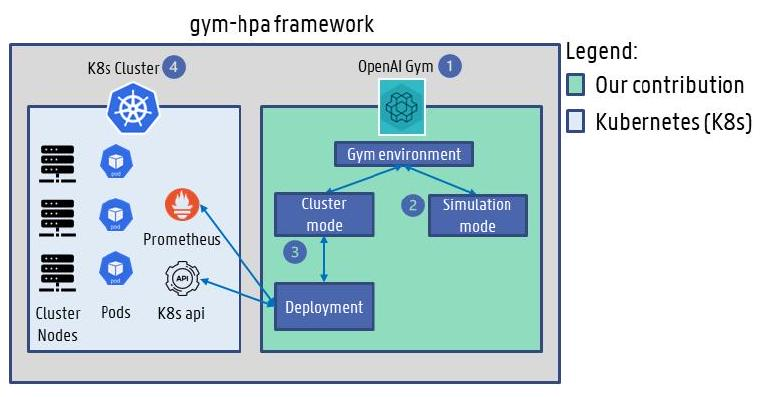
\includegraphics[width=\linewidth]{images/2024_11_17_21ad14b6196e5740bf69g-4}
    \caption{Overview of the k8s-hpa framework and its main components.}
    \label{fig:k8s-hpa-overview}
\end{figure}

\subsection{Kubernetes Integration}

Table~\ref{tab:k8s-deployment} describes the information available in the Deployment component of the k8s-hpa framework based on a Kubernetes deployment. The framework allows developers to specify the microservices $\mathcal{D}_a$ belonging to an application $a$. Input information (e.g., $P_d, N_a$) is retrieved from the K8s API, while current status metrics (e.g., $R_d, \rho_{d,[r]}$) are fetched using the Prometheus API.

An important Kubernetes concept is resource requests $\gamma_{d,[r]}$ and limitations $\Gamma_{d,[r]}$ \cite{kubernetes_resource_management}. Requests represent the minimum amount of resources (e.g., CPU, memory) needed by all containers in the pod, while limits correspond to the maximum resources allocated. Developers should specify these resource requests and limits to ensure Kubernetes schedules and auto-scales these pods appropriately. In the k8s-hpa framework, the desired number of replicas $R_d$ is calculated using resource requests and a default target resource utilization of 75\%.

\begin{table}[h]
    \centering
    \caption{Deployment status in the k8s-hpa framework.}
    \label{tab:k8s-deployment}
    \begin{tabular}{|c|l|}
        \hline
        \textbf{Symbol} & \textbf{Description} \\
        \hline
        $a$ & The application $a$. Each application consists of \\
        $D_a$ & different deployments $d \in D_a$. \\
        $N_a$ & Set of deployments belonging to application $a$. \\
        $C_d$ & Set of container names $c \in C$ for deployment $d$. \\
        $I_d$ & Set of container images $i \in I$ for deployment $d$. \\
        $P_d$ & Set of all pods belonging to deployment $d$. \\
        $\alpha_{d, \text{max}}$ & Maximum replicas allowed for deployment $d$. \\
        $\alpha_{d, \text{min}}$ & Minimum replicas allowed for deployment $d$. \\
        $\gamma_{d,[r]}$ & Request vector for deployment $d$. Resources: CPU (in m), \\
        & memory (in Mi). $m$: millicore, $Mi$: mebibyte. \\
        $\Gamma_{d,[r]}$ & Limit vector for deployment $d$. Resources as CPU (in m) \\
        & and memory (in Mi). \\
        $\rho_{d,[r]}$ & Total usage vector for deployment $d$ (CPU and memory). \\
        $\sigma_{d,i}$ & Total traffic received (in Kbps) by deployment $d$. \\
        $\Psi_a$ & Application latency (in ms). \\
        $R_d$ & Current number of deployed pods for deployment $d$. \\
        $\tau_a$ & Desired number of replicas for deployment $d$. \\
        $T$ & Resource usage threshold. Default: 0.75. \\
        $\Omega_c, \Omega_m$ & CPU and memory weights for replica calculation. Default: \\
        & $\Omega_c = 0.7, \Omega_m = 0.3$. \\
        \hline
    \end{tabular}
\end{table}

The default formula for calculating the desired number of replicas is provided in Equation~\ref{eq:replica-calculation}, considering multiple resource types. Optimal resource usage (e.g., 75\%) avoids performance degradation caused by overloading or resource contention.

\begin{equation}
    \tau_a = \left\lceil \Omega_c \cdot \omega_c + \Omega_m \cdot \omega_m \right\rceil
    \label{eq:replica-calculation}
\end{equation}

where $\omega_c$ and $\omega_m$ are the desired CPU and memory utilizations.

\section{Toward Efficient Auto-Scaling for Complex Microservice Applications in Kubernetes}
\label{sec:efficient_auto_scaling}

\subsection{Reinforcement Learning (RL)-based Auto-scaling}

Recently, Reinforcement Learning (RL) has become an important research field \cite{hessel2018rainbow}, often applied to solve sequential decision-making problems where agents learn actions directly from experience by interacting with an environment. Initially, the agent knows nothing about the given task and learns by receiving a reward for each action. The reward relates to the new observation, describing the environment state after applying the action selected by the agent.

In the context of auto-scaling, the agent receives a positive reward when an action increases application performance (e.g., high resource utilization, low response time). Conversely, the agent is penalized for degrading performance. Through repeated interactions, the agent learns to maximize long-term rewards by identifying synergies between states, actions, and rewards. RL is particularly well-suited for auto-scaling problems, as agents adapt their decisions to the evolving environment.

\subsection{Observation Space}

The observation space corresponds to the state of the environment at a given moment. Table~\ref{tab:observation-space} shows an example of the observation space for an application managed by the k8s-hpa framework. Each deployment in the application includes six metrics, such as the current number of deployed pods (`numPods`) and the desired number of replicas (`desiredReplicas`). These metrics provide the necessary context for the agent to select appropriate actions.

The observation space is retrieved either from the Kubernetes API and Prometheus API in cluster mode or simulated datasets in simulation mode.

\begin{table}[h]
    \centering
    \caption{Observation Space Structure of k8s-hpa.}
    \label{tab:observation-space}
    \begin{tabular}{|l|l|}
        \hline
        \textbf{Metric} & \textbf{Description} \\
        \hline
        numPods & Number of deployed pods. \\
        desiredReplicas & Desired number of replicas. \\
        cpuAggr & Total aggregated CPU (in m) of the pods. \\
        memAggr & Total aggregated memory (in Mi) of the pods. \\
        avgTrafficIn & Average received traffic (in Kbps). \\
        avgTrafficOut & Average transmitted traffic (in Kbps). \\
        \hline
    \end{tabular}
\end{table}

\subsection{Action Space}

The action space comprises all the possible actions that the agent can perform in the environment. Table~\ref{tab:action-space} shows a potential action space in the k8s-hpa framework for an application with two microservices. The action space is designed as \textit{MultiDiscrete} \cite{openAIGym}, meaning a list of possible actions exists for each microservice, and only one action is selected per step for each microservice.

The first discrete set corresponds to the selection of a microservice deployment (e.g., Deployment 1 or Deployment 2), and the second set corresponds to scaling actions. Agents can perform actions such as:
\begin{itemize}
    \item \textbf{DoNothing:} Keep the deployment as is.
    \item \textbf{Add:} Scale-out by deploying one or more replicas.
    \item \textbf{Stop:} Scale-in by terminating one or more replicas.
\end{itemize}

The range of actions depends on the maximum and minimum replica thresholds ($\alpha_{d,\text{max}}$ and $\alpha_{d,\text{min}}$) defined for each deployment.

\begin{table}[h]
    \centering
    \caption{Action Space Structure of k8s-hpa.}
    \label{tab:action-space}
    \begin{tabular}{|c|c|l|}
        \hline
        \textbf{Discrete Set} & \textbf{Action Name} & \textbf{Description} \\
        \hline
        Microservice & D1, D2 & Action triggered on Deployment 1 or 2. \\
        Scaling & DoNothing & No scaling action performed. \\
        & Add-1, Add-2, Add-3 & Add one, two, or three replicas. \\
        & Stop-1, Stop-2, Stop-3 & Remove one, two, or three replicas. \\
        \hline
    \end{tabular}
\end{table}

\subsection{Reward Function}

The reward function is a crucial component that guides the agent to maximize cumulative rewards by selecting appropriate actions. Two reward functions were designed to achieve distinct objectives:
\begin{itemize}
    \item \textbf{Cost Function:} This function encourages the agent to allocate the accurate number of replicas for each microservice deployment, focusing on reducing deployment costs by increasing resource utilization. The reward for this function is defined in Equation~\ref{eq:cost-reward}.
    \item \textbf{Latency Function:} This function penalizes the agent based on application latency, encouraging the agent to allocate resources to keep latency below a threshold. The reward for this function is defined in Equation~\ref{eq:latency-reward}.
\end{itemize}

\begin{equation}
    \text{getCostReward}(d) =
    \begin{cases} 
        1.0 & \text{if } R_d = \omega_d, \\
        0 & \text{otherwise.}
    \end{cases}
    \label{eq:cost-reward}
\end{equation}

\begin{equation}
    \text{getLatencyReward}(a) =
    \begin{cases}
        -\Psi_a & \text{if } \Psi_a \leq \tau_a, \\
        -\tau_a & \text{otherwise.}
    \end{cases}
    \label{eq:latency-reward}
\end{equation}

The cost function assigns a positive reward when the number of deployed replicas matches the desired value. Any attempt to violate minimum or maximum replica thresholds results in a penalty.

The latency function penalizes the agent linearly based on the application's latency ($\Psi_a$). The threshold $\tau_a$ defines the maximum acceptable latency, beyond which a fixed penalty is applied. Both functions follow a linear reward pattern, simplifying the learning process for the agent.

\subsection{Agents}

The k8s-hpa framework supports RL agents implemented using the Stable Baselines 3 \cite{raffin2019stable} library, which provides reliable implementations of RL algorithms. Two specific RL agents were evaluated:

\begin{itemize}
    \item \textbf{Advantage Actor-Critic (A2C):} A synchronous, deterministic algorithm that combines policy and value-based methods. Policy-based agents directly map states to actions (i.e., actors), while value-based methods evaluate the quality of actions (i.e., critics). A2C uses a single thread to compute gradients, ensuring determinism.
    \item \textbf{Recurrent Proximal Policy Optimization (RPPO):} Similar to Proximal Policy Optimization (PPO), a widely used policy gradient method, RPPO extends PPO by adding support for recurrent policies like Long Short-Term Memory (LSTM). This enables RPPO to incorporate historical information into its decision-making process, improving performance in environments with temporal dependencies.
\end{itemize}

The agents interact with the k8s-hpa framework by selecting actions based on the observed state of the environment and the defined reward function. Both agents can handle the multi-discrete action space presented earlier, allowing them to scale multiple microservices simultaneously.


\section{Evaluation Setup}
\label{sec:evaluation_setup}
\subsection{Applications}

The evaluation setup considers two microservice-based applications for training and testing RL agents within the k8s-hpa framework. Table~\ref{tab:application-deployments} summarizes the properties of these applications, including deployment configurations and resource constraints.

\paragraph{Redis Cluster (RC)} 
The Redis Cluster application (Figure~\ref{fig:redis-cluster}) consists of two Kubernetes deployments: \textit{master} and \textit{slave}. It represents a database application where the Redis-benchmark utility \cite{redisBenchmark} generates database queries from emulated clients during RL training and testing. The number of emulated clients dynamically varies to ensure the RL agents adapt their scaling decisions to changing demands. The Redis Exporter \cite{redisExporter}, integrated with Prometheus, monitors performance metrics like CPU usage and response time.

The latency for the RC application, denoted as $\Psi_{a_1}$, is calculated as the average query response time over a 5-minute window. Equation~\ref{eq:redis-latency} defines this calculation:

\begin{equation}
    \Psi_{a_1} = \frac{\text{redis\_commands\_duration\_seconds\_total}[5\text{m}]}{\text{redis\_commands\_processed\_total}[5\text{m}]}
    \label{eq:redis-latency}
\end{equation}

The latency threshold $\tau_{a_1}$ is set at 250 milliseconds (ms).

\begin{figure}[h]
    \centering
    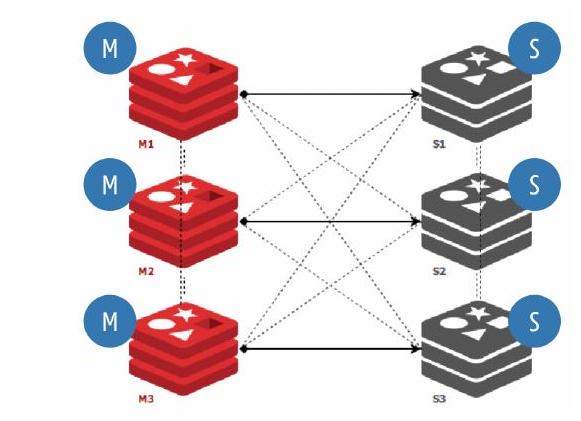
\includegraphics[width=0.8\linewidth]{images/2024_11_17_21ad14b6196e5740bf69g-6(1)}
    \caption{Illustration of the Redis Cluster (RC) application.}
    \label{fig:redis-cluster}
\end{figure}

\paragraph{Online Boutique (OB)}
The Online Boutique application (Figure~\ref{fig:online-boutique}) is a web-based e-commerce platform with 11 Kubernetes deployments, including services like \textit{Frontend}, \textit{Cart}, \textit{Checkout}, and \textit{Recommendation}. Users browse items, add them to their cart, and proceed to purchase. RL training is driven by simulated workloads using the Locust load testing tool \cite{locust}, which generates a mix of GET and POST requests.

The latency for OB, denoted as $\Psi_{a_2}$, is derived from the average response time for the \texttt{GET /cart} request. Equation~\ref{eq:ob-latency} defines this calculation:

\begin{equation}
    \Psi_{a_2} = \text{locust\_avg\_response\_time\_GET\_cart}
    \label{eq:ob-latency}
\end{equation}

The latency threshold $\tau_{a_2}$ is set at 3 seconds (3000 ms).

\begin{figure}[h]
    \centering
    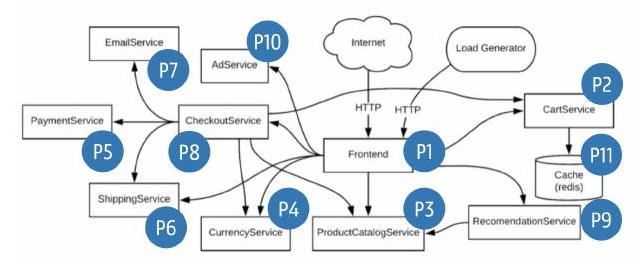
\includegraphics[width=0.8\linewidth]{images/2024_11_17_21ad14b6196e5740bf69g-6}
    \caption{Illustration of the Online Boutique (OB) application.}
    \label{fig:online-boutique}
\end{figure}

\begin{table}[h]
    \centering
    \caption{Deployment properties of the evaluated applications.}
    \label{tab:application-deployments}
    \begin{tabular}{|c|c|c|c|c|}
        \hline
        \textbf{Application} & \textbf{Deployment} & \textbf{CPU R/L (m)} & \textbf{RAM R/L (Mi)} & \textbf{Min/Max Replicas} \\
        \hline
        \multirow{2}{*}{Redis Cluster} 
            & Master & 250 / 500 & 250 / 500 & 1 / 8 \\
            & Slave  & 250 / 500 & 250 / 500 & 1 / 8 \\
        \hline
        \multirow{11}{*}{Online Boutique} 
            & Frontend & 100 / 200 & 64 / 128 & 1 / 8 \\
            & Cart     & 200 / 300 & 180 / 300 & 1 / 8 \\
            & Product  & 100 / 200 & 64 / 128 & 1 / 8 \\
            & Currency & 100 / 200 & 64 / 128 & 1 / 8 \\
            & Payment  & 100 / 200 & 64 / 128 & 1 / 8 \\
            & Shipping & 100 / 200 & 64 / 128 & 1 / 8 \\
            & Email    & 100 / 200 & 64 / 128 & 1 / 8 \\
            & Checkout & 100 / 200 & 64 / 128 & 1 / 8 \\
            & Recommend. & 100 / 200 & 64 / 128 & 1 / 8 \\
            & Ad       & 200 / 300 & 180 / 300 & 1 / 8 \\
            & Redis-cart & 70 / 125 & 200 / 256 & 1 / 8 \\
        \hline
    \end{tabular}
\end{table}

\subsection{Dataset Creation}

Datasets for both Redis Cluster (RC) and Online Boutique (OB) applications were collected from real Kubernetes deployments. These datasets are essential for the simulation mode, enabling near-real training environments for RL agents. The data represent the actual resource usage and performance metrics of these applications under varying workloads.

\paragraph{Redis Cluster (RC)}
For the RC application, the dataset includes:
\begin{itemize}
    \item Number of deployed pods.
    \item Aggregated CPU and memory usage.
    \item Query response times.
    \item Received and transmitted traffic.
\end{itemize}
The data were collected while generating database queries using the Redis-benchmark utility \cite{redisBenchmark}. The cumulative distribution of CPU usage for the \textit{master} deployment is shown in Figure~\ref{fig:redis-cdf}. This data helps simulate realistic responses for varying workloads.

\paragraph{Online Boutique (OB)}
For the OB application, datasets were created using the Locust load testing tool \cite{locust}, which emulates user interactions with the e-commerce platform. The data include:
\begin{itemize}
    \item Number of deployed pods for each service.
    \item Aggregated CPU and memory usage.
    \item Average response times for specific requests.
    \item Traffic patterns for incoming and outgoing HTTP requests.
\end{itemize}
This dataset enables the RL agents to evaluate scaling actions in scenarios of fluctuating user demand.

\begin{figure}[h]
    \centering
    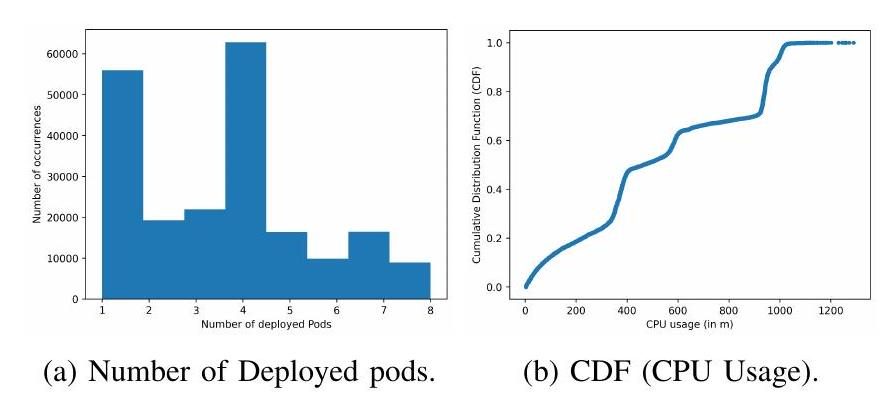
\includegraphics[width=0.8\linewidth]{images/2024_11_17_21ad14b6196e5740bf69g-7(2)}
    \caption{Analysis of the Redis Cluster (RC) master deployment: Cumulative Distribution Function (CDF) of CPU usage.}
    \label{fig:redis-cdf}
\end{figure}

\paragraph{Simulation Mode}
In the simulation mode, observations are retrieved directly from these datasets. For each action selected by the RL agent, the framework fetches the corresponding state from the dataset. This approach ensures that the simulation reflects near-real behaviors while avoiding the overhead of interacting with an actual Kubernetes cluster.

\subsection{Testbed Implementation}

The k8s-hpa framework has been implemented in Python to simplify interaction with both the OpenAI Gym library and the Stable Baselines 3 library \cite{raffin2019stable}. The Kubernetes Python Client was used to interface with a Kubernetes cluster, retrieving information about deployments and metrics via the Kubernetes and Prometheus APIs.

\paragraph{Hardware and Software Setup}
The evaluation environment was deployed on a machine with the following specifications:
\begin{itemize}
    \item \textbf{Processor:} 14-core Intel i7-12700H CPU @ 4.7 GHz.
    \item \textbf{Memory:} 16 GB RAM.
    \item \textbf{Operating System:} Ubuntu 20.04.2 LTS.
\end{itemize}

Table~\ref{tab:testbed-software} summarizes the software versions used in the experiments.

\begin{table}[h]
    \centering
    \caption{Software versions of the testbed.}
    \label{tab:testbed-software}
    \begin{tabular}{|l|l|}
        \hline
        \textbf{Software} & \textbf{Version} \\
        \hline
        Python \& Kubernetes Python Client & 3.10 \& 23.6.0 \\
        Gym \& Stable Baselines 3 & 0.21.0 \& 1.5.0 \\
        Kubeadm \& Kubectl & v1.22.4 \\
        Docker \& Linux Kernel & docker://20.10.10 \& 5.4.0-80-generic \\
        Operating System & Ubuntu 20.04.2 LTS \\
        \hline
    \end{tabular}
\end{table}

\paragraph{Training Configuration}
The RL agents were trained in episodes, where each episode consisted of 25 steps. At each step, the agent attempted to maximize rewards by selecting appropriate scaling actions based on the current environment state. Two RL agents—A2C and RPPO—were trained with their default parameters from the Stable Baselines 3 library.

The training environment configurations for the Redis Cluster and Online Boutique applications are shown in Table~\ref{tab:environment-config}.

\begin{table}[h]
    \centering
    \caption{Environment configurations for k8s-hpa.}
    \label{tab:environment-config}
    \begin{tabular}{|c|c|c|c|}
        \hline
        \textbf{Name} & \textbf{Deployments} & \textbf{Action Space} & \textbf{Observation Space} \\
        \hline
        Redis Cluster & 2 & MultiDiscrete(2,15) & 20 states \\
        Online Boutique & 11 & MultiDiscrete(11,15) & 110 states \\
        \hline
    \end{tabular}
\end{table}

\paragraph{Execution Details}
In the evaluation, the simulation mode provided near-real metrics to train the RL agents efficiently. Cluster mode was used for validation, ensuring the agents performed effectively under actual Kubernetes conditions. Each RL algorithm was executed for 2000 episodes, with a focus on either reducing costs or minimizing application latency.


\section{Results}
\label{sec:results}
This section presents the results obtained during the training and testing phases of the RL agents, evaluated in both simulation and cluster modes. Key metrics include execution time, accumulated rewards, the number of deployed pods, and application latency.

\subsection{Training Phase}

The execution time per episode (25 steps) during training is shown in Table~\ref{tab:training-time}. The simulation mode is significantly faster since observations are retrieved from datasets rather than being fetched via the Kubernetes and Prometheus APIs in cluster mode.

\begin{table}[h]
    \centering
    \caption{Execution time per episode during training.}
    \label{tab:training-time}
    \begin{tabular}{|c|c|c|c|}
        \hline
        \textbf{Algorithm} & \textbf{Application} & \textbf{Mode} & \textbf{Execution Time (s)} \\
        \hline
        A2C & Redis Cluster & Simulation & $0.445 \pm 0.252$ \\
        RPPO & Redis Cluster & Simulation & $0.600 \pm 0.300$ \\
        A2C & Redis Cluster & Cluster & $20.090 \pm 6.833$ \\
        RPPO & Redis Cluster & Cluster & $24.968 \pm 8.865$ \\
        A2C & Online Boutique & Simulation & $1.262 \pm 0.146$ \\
        RPPO & Online Boutique & Simulation & $1.890 \pm 1.177$ \\
        A2C & Online Boutique & Cluster & $226.300 \pm 58.680$ \\
        RPPO & Online Boutique & Cluster & $285.963 \pm 91.229$ \\
        \hline
    \end{tabular}
\end{table}

Figures~\ref{fig:rc-rewards} and \ref{fig:ob-rewards} illustrate the accumulated rewards during training for the Redis Cluster and Online Boutique applications, respectively. For the Redis Cluster, the cluster mode achieves slightly higher rewards for the cost function. For the latency function, both simulation and cluster modes guide the agent to find optimal scaling actions to minimize latency penalties.

\begin{figure}[h]
    \centering
    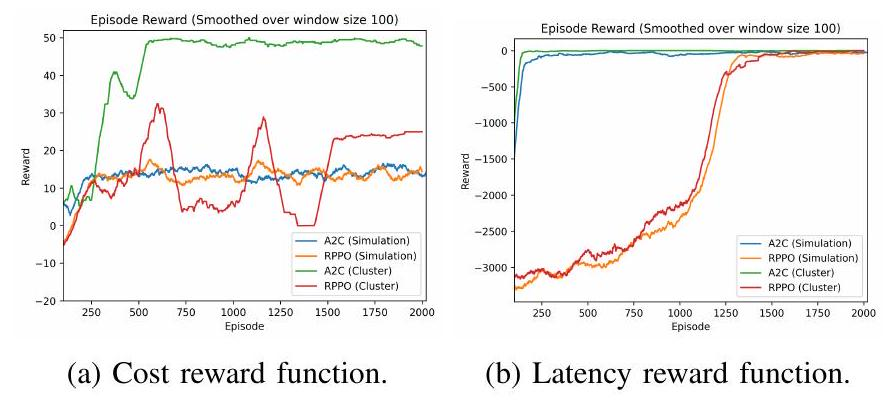
\includegraphics[width=0.8\linewidth]{images/2024_11_17_21ad14b6196e5740bf69g-7}
    \caption{Accumulated rewards during training for the Redis Cluster (RC) application.}
    \label{fig:rc-rewards}
\end{figure}

\begin{figure}[h]
    \centering
    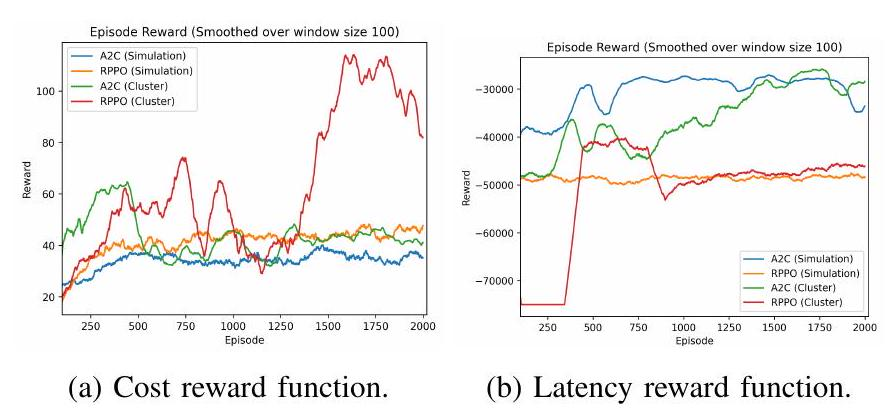
\includegraphics[width=0.8\linewidth]{images/2024_11_17_21ad14b6196e5740bf69g-7(1)}
    \caption{Accumulated rewards during training for the Online Boutique (OB) application.}
    \label{fig:ob-rewards}
\end{figure}

\subsection{Testing Phase}

During the testing phase, RL agents were executed for 100 episodes using the configurations saved after 2000 training episodes. Key metrics include accumulated rewards, the average number of deployed pods, and application latency. Table~\ref{tab:testing-results} summarizes the results for both Redis Cluster and Online Boutique applications.

\begin{table}[h]
    \centering
    \caption{Results obtained during the testing phase.}
    \label{tab:testing-results}
    \begin{tabular}{|c|c|c|c|c|c|}
        \hline
        \multicolumn{6}{|c|}{\textbf{Redis Cluster (RC) Application}} \\
        \hline
        \textbf{Algorithm} & \textbf{Mode} & \textbf{Goal} & \textbf{Reward} & \textbf{Pods} & \textbf{Latency ($\mu$s)} \\
        \hline
        A2C & Simulation & Cost & $24.6 \pm 2.9$ & $2.3 \pm 0.4$ & $55.3 \pm 8.7$ \\
        RPPO & Simulation & Cost & $26.3 \pm 6.7$ & $2.8 \pm 0.8$ & $107.9 \pm 59.8$ \\
        A2C & Cluster & Cost & $24.0 \pm 3.2$ & $2.4 \pm 0.6$ & $36.6 \pm 18.2$ \\
        RPPO & Cluster & Cost & $24.2 \pm 3.0$ & $2.2 \pm 0.3$ & $46.2 \pm 12.1$ \\
        A2C & Simulation & Latency & $-0.4 \pm 0.1$ & $3.3 \pm 0.9$ & $15.1 \pm 1.5$ \\
        RPPO & Simulation & Latency & $-0.9 \pm 2.8$ & $3.6 \pm 0.7$ & $23.5 \pm 6.0$ \\
        A2C & Cluster & Latency & $-1.7 \pm 2.9$ & $13.3 \pm 2.0$ & $28.3 \pm 15.0$ \\
        RPPO & Cluster & Latency & $-7.0 \pm 36.0$ & $8.4 \pm 4.4$ & $42.4 \pm 11.2$ \\
        \hline
        KHPA & - & CPU Usage & - & $4.1 \pm 0.9$ & $44.8 \pm 34.2$ \\
        \hline
        \multicolumn{6}{|c|}{\textbf{Online Boutique (OB) Application}} \\
        \hline
        \textbf{Algorithm} & \textbf{Mode} & \textbf{Goal} & \textbf{Reward} & \textbf{Pods} & \textbf{Latency (s)} \\
        \hline
        A2C & Simulation & Cost & $83.2 \pm 59.7$ & $14.9 \pm 3.0$ & $1.05 \pm 0.48$ \\
        RPPO & Simulation & Cost & $124.8 \pm 27.2$ & $14.9 \pm 3.1$ & $1.09 \pm 0.27$ \\
        A2C & Cluster & Cost & $153.6 \pm 32.2$ & $13.1 \pm 3.2$ & $1.28 \pm 0.39$ \\
        RPPO & Cluster & Cost & $113.7 \pm 41.3$ & $24.8 \pm 8.6$ & $1.17 \pm 0.42$ \\
        A2C & Simulation & Latency & $-25.6K \pm 3.3K$ & $43.4 \pm 9.6$ & $0.92 \pm 0.16$ \\
        RPPO & Simulation & Latency & $-71.2K \pm 9.9K$ & $50.7 \pm 6.8$ & $1.08 \pm 0.25$ \\
        A2C & Cluster & Latency & $-34.4K \pm 6.2K$ & $54.5 \pm 8.6$ & $0.98 \pm 0.52$ \\
        RPPO & Cluster & Latency & $-60.3K \pm 8.6K$ & $46.3 \pm 6.5$ & $0.99 \pm 0.19$ \\
        \hline
        KHPA & - & CPU Usage & - & $16.7 \pm 3.7$ & $1.22 \pm 0.21$ \\
        \hline
    \end{tabular}
\end{table}

\subsection{Analysis}

The results demonstrate the following key points:
\begin{itemize}
    \item RL-based approaches (A2C and RPPO) significantly reduce deployment costs and application latency compared to KHPA, which does not consider microservice interdependencies.
    \item A2C outperformed RPPO in latency reduction for the Online Boutique application.
    \item Simulation mode enables efficient training, while cluster mode validates real-world effectiveness.
\end{itemize}

\section{Conclusion}
\label{sec:conclusion}
This paper presents the k8s-hpa framework, which bridges the gap between Reinforcement Learning (RL) and auto-scaling research for Kubernetes-based microservice applications. The framework leverages the OpenAI Gym library and Kubernetes platform to create a suitable environment for RL agents to learn optimal scaling actions. By addressing microservice interdependencies and application performance, k8s-hpa provides an innovative approach to auto-scaling that goes beyond traditional threshold-based methods.

Experiments conducted with the Redis Cluster (RC) and Online Boutique (OB) applications demonstrated significant improvements:
\begin{itemize}
    \item RL agents trained with k8s-hpa reduced resource usage by at least 30\% compared to default Kubernetes Horizontal Pod Autoscaler (KHPA).
    \item Application latency was reduced by up to 25\%, highlighting the framework's ability to meet performance requirements under dynamic workloads.
\end{itemize}

The framework has been released as open-source software to facilitate further research in RL-based auto-scaling. Future work will focus on developing multi-objective RL agents capable of balancing competing goals such as cost efficiency, latency reduction, and fault tolerance. Additionally, the integration of vertical scaling and hybrid elasticity approaches will be explored to address resource allocation challenges in next-generation cloud platforms.


\section*{References}

% \bibliographystyle{abbrv}
\bibliographystyle{IEEEtran}

\bibliography{references}

\end{document}
